\PassOptionsToPackage{unicode=true}{hyperref} % options for packages loaded elsewhere
\PassOptionsToPackage{hyphens}{url}
%
\documentclass[]{book}
\usepackage{lmodern}
\usepackage{amssymb,amsmath}
\usepackage{ifxetex,ifluatex}
\usepackage{fixltx2e} % provides \textsubscript
\ifnum 0\ifxetex 1\fi\ifluatex 1\fi=0 % if pdftex
  \usepackage[T1]{fontenc}
  \usepackage[utf8]{inputenc}
  \usepackage{textcomp} % provides euro and other symbols
\else % if luatex or xelatex
  \usepackage{unicode-math}
  \defaultfontfeatures{Ligatures=TeX,Scale=MatchLowercase}
\fi
% use upquote if available, for straight quotes in verbatim environments
\IfFileExists{upquote.sty}{\usepackage{upquote}}{}
% use microtype if available
\IfFileExists{microtype.sty}{%
\usepackage[]{microtype}
\UseMicrotypeSet[protrusion]{basicmath} % disable protrusion for tt fonts
}{}
\IfFileExists{parskip.sty}{%
\usepackage{parskip}
}{% else
\setlength{\parindent}{0pt}
\setlength{\parskip}{6pt plus 2pt minus 1pt}
}
\usepackage{hyperref}
\hypersetup{
            pdftitle={The BOAST Style Guide},
            pdfauthor={Neil Hatfield (njh5464@psu.edu) and Robert Carey (rpc5102@psu.edu)},
            pdfborder={0 0 0},
            breaklinks=true}
\urlstyle{same}  % don't use monospace font for urls
\usepackage{color}
\usepackage{fancyvrb}
\newcommand{\VerbBar}{|}
\newcommand{\VERB}{\Verb[commandchars=\\\{\}]}
\DefineVerbatimEnvironment{Highlighting}{Verbatim}{commandchars=\\\{\}}
% Add ',fontsize=\small' for more characters per line
\usepackage{framed}
\definecolor{shadecolor}{RGB}{248,248,248}
\newenvironment{Shaded}{\begin{snugshade}}{\end{snugshade}}
\newcommand{\AlertTok}[1]{\textcolor[rgb]{0.94,0.16,0.16}{#1}}
\newcommand{\AnnotationTok}[1]{\textcolor[rgb]{0.56,0.35,0.01}{\textbf{\textit{#1}}}}
\newcommand{\AttributeTok}[1]{\textcolor[rgb]{0.77,0.63,0.00}{#1}}
\newcommand{\BaseNTok}[1]{\textcolor[rgb]{0.00,0.00,0.81}{#1}}
\newcommand{\BuiltInTok}[1]{#1}
\newcommand{\CharTok}[1]{\textcolor[rgb]{0.31,0.60,0.02}{#1}}
\newcommand{\CommentTok}[1]{\textcolor[rgb]{0.56,0.35,0.01}{\textit{#1}}}
\newcommand{\CommentVarTok}[1]{\textcolor[rgb]{0.56,0.35,0.01}{\textbf{\textit{#1}}}}
\newcommand{\ConstantTok}[1]{\textcolor[rgb]{0.00,0.00,0.00}{#1}}
\newcommand{\ControlFlowTok}[1]{\textcolor[rgb]{0.13,0.29,0.53}{\textbf{#1}}}
\newcommand{\DataTypeTok}[1]{\textcolor[rgb]{0.13,0.29,0.53}{#1}}
\newcommand{\DecValTok}[1]{\textcolor[rgb]{0.00,0.00,0.81}{#1}}
\newcommand{\DocumentationTok}[1]{\textcolor[rgb]{0.56,0.35,0.01}{\textbf{\textit{#1}}}}
\newcommand{\ErrorTok}[1]{\textcolor[rgb]{0.64,0.00,0.00}{\textbf{#1}}}
\newcommand{\ExtensionTok}[1]{#1}
\newcommand{\FloatTok}[1]{\textcolor[rgb]{0.00,0.00,0.81}{#1}}
\newcommand{\FunctionTok}[1]{\textcolor[rgb]{0.00,0.00,0.00}{#1}}
\newcommand{\ImportTok}[1]{#1}
\newcommand{\InformationTok}[1]{\textcolor[rgb]{0.56,0.35,0.01}{\textbf{\textit{#1}}}}
\newcommand{\KeywordTok}[1]{\textcolor[rgb]{0.13,0.29,0.53}{\textbf{#1}}}
\newcommand{\NormalTok}[1]{#1}
\newcommand{\OperatorTok}[1]{\textcolor[rgb]{0.81,0.36,0.00}{\textbf{#1}}}
\newcommand{\OtherTok}[1]{\textcolor[rgb]{0.56,0.35,0.01}{#1}}
\newcommand{\PreprocessorTok}[1]{\textcolor[rgb]{0.56,0.35,0.01}{\textit{#1}}}
\newcommand{\RegionMarkerTok}[1]{#1}
\newcommand{\SpecialCharTok}[1]{\textcolor[rgb]{0.00,0.00,0.00}{#1}}
\newcommand{\SpecialStringTok}[1]{\textcolor[rgb]{0.31,0.60,0.02}{#1}}
\newcommand{\StringTok}[1]{\textcolor[rgb]{0.31,0.60,0.02}{#1}}
\newcommand{\VariableTok}[1]{\textcolor[rgb]{0.00,0.00,0.00}{#1}}
\newcommand{\VerbatimStringTok}[1]{\textcolor[rgb]{0.31,0.60,0.02}{#1}}
\newcommand{\WarningTok}[1]{\textcolor[rgb]{0.56,0.35,0.01}{\textbf{\textit{#1}}}}
\usepackage{longtable,booktabs}
% Fix footnotes in tables (requires footnote package)
\IfFileExists{footnote.sty}{\usepackage{footnote}\makesavenoteenv{longtable}}{}
\usepackage{graphicx,grffile}
\makeatletter
\def\maxwidth{\ifdim\Gin@nat@width>\linewidth\linewidth\else\Gin@nat@width\fi}
\def\maxheight{\ifdim\Gin@nat@height>\textheight\textheight\else\Gin@nat@height\fi}
\makeatother
% Scale images if necessary, so that they will not overflow the page
% margins by default, and it is still possible to overwrite the defaults
% using explicit options in \includegraphics[width, height, ...]{}
\setkeys{Gin}{width=\maxwidth,height=\maxheight,keepaspectratio}
\usepackage[normalem]{ulem}
% avoid problems with \sout in headers with hyperref:
\pdfstringdefDisableCommands{\renewcommand{\sout}{}}
\setlength{\emergencystretch}{3em}  % prevent overfull lines
\providecommand{\tightlist}{%
  \setlength{\itemsep}{0pt}\setlength{\parskip}{0pt}}
\setcounter{secnumdepth}{5}
% Redefines (sub)paragraphs to behave more like sections
\ifx\paragraph\undefined\else
\let\oldparagraph\paragraph
\renewcommand{\paragraph}[1]{\oldparagraph{#1}\mbox{}}
\fi
\ifx\subparagraph\undefined\else
\let\oldsubparagraph\subparagraph
\renewcommand{\subparagraph}[1]{\oldsubparagraph{#1}\mbox{}}
\fi

% set default figure placement to htbp
\makeatletter
\def\fps@figure{htbp}
\makeatother

\usepackage{booktabs}
\usepackage{amsthm}
\makeatletter
\def\thm@space@setup{%
  \thm@preskip=8pt plus 2pt minus 4pt
  \thm@postskip=\thm@preskip
}
\makeatother
\usepackage[]{natbib}
\bibliographystyle{apalike}

\title{The BOAST Style Guide}
\author{Neil Hatfield (\href{mailto:njh5464@psu.edu}{\nolinkurl{njh5464@psu.edu}}) and Robert Carey (\href{mailto:rpc5102@psu.edu}{\nolinkurl{rpc5102@psu.edu}})}
\date{21 May 2020}

\begin{document}
\maketitle

{
\setcounter{tocdepth}{1}
\tableofcontents
}
\hypertarget{welcome}{%
\chapter{Welcome}\label{welcome}}

This guide spells out the styling that should be used for all apps included in \href{https://github.com/EducationShinyAppTeam/BOAST}{BOAST}. Keep in mind that there are several different aspects to what makes up Style including:

\begin{itemize}
\tightlist
\item
  Coding (how you write, organize, and comment the code that makes the app)
\item
  Visual Appearance (how you make the app look including tabs, fonts, colors, icons, etc.)
\item
  Wording (how you write information, instructions, and other messages to the users)
\item
  Documentation (how you provide references, including code and data sources, and give credit)
\end{itemize}

By following this style guide you'll ensure that any app you create will
meet our standards.

\hypertarget{getStarted}{%
\chapter{Getting Started}\label{getStarted}}

Before you get too far into the Style Guide, we would like for you to take a moment and ensure that you have the following tools at your disposal.

\hypertarget{checklist}{%
\section{Getting Started Checklist}\label{checklist}}

\begin{enumerate}
\def\labelenumi{\arabic{enumi}.}
\tightlist
\item
  Ensure that you have all of necessary accounts and if not, put in a request to Robert (Bob).

  \begin{enumerate}
  \def\labelenumii{\alph{enumii}.}
  \tightlist
  \item
    DataCamp\\
  \item
    GitHub\\
  \item
    EducationShinyAppTeam on GitHub\\
  \item
    \sout{RStudio Server}

    \begin{itemize}
    \tightlist
    \item
      Upon investigation the TLT and the Eberly RStudio Servers will not be useful for us to do testing. An alternate testing process will be explored.\\
    \end{itemize}
  \item
    BOAST in Teams (tied to your PSU ID)
  \end{enumerate}
\item
  Ensure that you have all of the proper software.

  \begin{enumerate}
  \def\labelenumii{\alph{enumii}.}
  \tightlist
  \item
    \texttt{R} (version 3.5.* minimum, version 4.0.0 preferred)\\
  \item
    RStudio (most current version preferred)\\
  \end{enumerate}
\item
  Additional Software that we recommend

  \begin{enumerate}
  \def\labelenumii{\alph{enumii}.}
  \tightlist
  \item
    GitHub Desktop\\
  \end{enumerate}
\item
  \texttt{R} Packages--here are some basic packages that everyone will need; be sure to install their dependencies too\\
\end{enumerate}

\begin{enumerate}
\def\labelenumi{\alph{enumi}.}
\tightlist
\item
  \texttt{tidyverse}~\\
\item
  \texttt{ggplot2}~\\
\item
  \texttt{shiny}~\\
\item
  \texttt{shinyBS}~\\
\item
  \texttt{boastUtils} (see below)\\
\end{enumerate}

\begin{enumerate}
\def\labelenumi{\arabic{enumi}.}
\setcounter{enumi}{4}
\tightlist
\item
  A copy of the Sample App (see below)
\end{enumerate}

\hypertarget{boastutils-package}{%
\section{\texorpdfstring{\texttt{boastUtils} Package}{boastUtils Package}}\label{boastutils-package}}

Bob created the \href{https://github.com/EducationShinyAppTeam/boastUtils}{boastUtils} package to automate much of the design and development process. This will not only reduce the amount of work you'll need to do, it'll also make apps more consistent.

\textbf{Starting Summer 2020, you will be required to you make use of this tool.}

Please check out the package's \href{https://github.com/EducationShinyAppTeam/boastUtils}{page} for instructions on installing and usage.

\hypertarget{sample-app}{%
\section{Sample App}\label{sample-app}}

Bob and Neil have created a Sample App repository that you can use as a template for your own apps. To get started, clone the \href{https://github.com/EducationShinyAppTeam/Sample_App}{Sample\_App} template repo found on GitHub. This will provide you with a skeleton for organizing your files as well as your code. There are several methods you can use:

\hypertarget{command-line}{%
\subsection{Command Line}\label{command-line}}

Enter the following in your terminal:

\begin{Shaded}
\begin{Highlighting}[]
\FunctionTok{git}\NormalTok{ clone git@github.com:EducationShinyAppTeam/Sample_App.git}
\end{Highlighting}
\end{Shaded}

\hypertarget{direct-download}{%
\subsection{Direct Download}\label{direct-download}}

You can download the repository directly:

\begin{quote}
\url{https://github.com/EducationShinyAppTeam/Sample_App/archive/master.zip}
\end{quote}

\hypertarget{github-desktop}{%
\subsection{GitHub Desktop}\label{github-desktop}}

If you are using GitHub Desktop and have linked your account that has access to the EducationShinyAppTeam repository, you can do the following from inside GitHub Desktop:

\begin{enumerate}
\def\labelenumi{\arabic{enumi}.}
\tightlist
\item
  Bring up the Clone Repository Menu (File -\textgreater{} Clone Repository\ldots{})\\
\item
  Enter Sample\_App in the search bar and select the option that says Sample\_App (not sampleapp)
\item
  Click the Choose\ldots{} button for the local path (this is where you want to the clone to live on your computer)
\item
  Click the Clone button.
\end{enumerate}

\hypertarget{coding}{%
\chapter{Coding Style}\label{coding}}

Now that you've gone through the Getting Started section, we can turn our attention to the first part of the Style Guide: Coding. There are many aspects that fall under the heading of Coding Style.

\hypertarget{genCode}{%
\section{General Coding Style}\label{genCode}}

Our general practice is to make use of the \href{https://style.tidyverse.org/}{tidyverse style guide}. However, we do have some important departures and additional practices you need to follow:

\hypertarget{comments}{%
\subsection{Leave Comments}\label{comments}}

At bare minimum, use a comment to break your code into sections. This helps you and others conceptualize the code into more manageable chunks. Your comments can provide others with potential keywords to search for when looking at your code later on.

For particularly complex sections, use comments to summarize what you're trying to do. This can help you and others pick up the coding thread for what you are trying to do for troubleshooting, debugging, and future improvements.

\hypertarget{naming}{%
\subsection{Informative Names}\label{naming}}

Use Informative Names for Variables and Functions in your code. Use names that give another person a sense of what that variable represents (nouns) or what the function is supposed to do (action verbs). For example,

\begin{itemize}
\tightlist
\item
  \texttt{scoreMatrix} is a matrix that holds a set of scores\\
\item
  \texttt{checkGame} is a function that checks the state of the current game
\end{itemize}

Use \textbf{camelCase} for variables and functions. The first word begins with a lowercase letter and additional words start with Capital letters with no space or underscore ( \_ ) between them. (This is a departure from the tidyverse style.)

Avoid using the variable names that existed in code you're making use of from another app or script. For example, don't use \texttt{waitTimes} to hold your data on the number of correct answers a user has given.

\hypertarget{formatCode}{%
\subsection{Format Your Code}\label{formatCode}}

See also \ref{orgCode} Organizing Code

Use indentation spacing to help make your code readable. RStudio has a built-in tool that can help with this.

\begin{enumerate}
\def\labelenumi{\arabic{enumi}.}
\tightlist
\item
  Select all of the code you want to reformat.

  \begin{itemize}
  \tightlist
  \item
    To select all code in a file, use Command-A (Mac) or Control-A (Windows).
  \end{itemize}
\item
  Press Command-Shift-A (Mac), Control-Shift-A (Windows), or click on the Code menu and select Reformat Code.
\end{enumerate}

NOTE: this tool is imperfect and can result in left parenthesis or curly braces moving up a line to where you might have an end-of-line comment, resulting in errors.

Additionally, you can make use of the \texttt{styler} and \texttt{lintr} packages to help you perform formatting checks and to quickly reformat code.

\hypertarget{explicit}{%
\subsection{Be Explicit}\label{explicit}}

One of the best practices a coder can do is to be explicit. This links back to Informative Naming (\ref{naming}) but goes a step beyond. \texttt{R} is a functional programming language. One of the important aspects of this is that functions in \texttt{R} obey the same rules as mathematical functions, especially multivariate functions.

One implicit fact about functions that most students don't realize is that the order of a function's arguments are a matter of convention and are actually arbitrary. While we might define \emph{f} as \(f(x,y) = x^2+3y\), we could call \(f(y=2,x=1)\) and get the same output as \(f(1,2)\) when we use the convention set up in the definition. This issue is exacerbated with functions in \texttt{R}.

Therefore, when you pass values to the arguments of a function in \texttt{R}, you should be explicit and include the argument name in your code. For example,

\begin{Shaded}
\begin{Highlighting}[]
\KeywordTok{actionButton}\NormalTok{(}
  \DataTypeTok{inputId =} \StringTok{"submit"}\NormalTok{,}
  \DataTypeTok{label =} \StringTok{"Submit"}\NormalTok{,}
  \DataTypeTok{color =} \StringTok{"primary"}\NormalTok{,}
  \DataTypeTok{style =} \StringTok{"bordered"}\NormalTok{,}
  \DataTypeTok{class =} \StringTok{"btn-ttt"}
\NormalTok{)}
\end{Highlighting}
\end{Shaded}

There are a few exceptions to this:

\begin{itemize}
\tightlist
\item
  Formula Arguments (e.g., \texttt{response\ \textasciitilde{}\ factor1\ +\ block})
\item
  Data Vectors/Frames (e.g., \texttt{dataFrame\$response})
\item
  Functions from \texttt{shiny}, \texttt{shinydashboard}, \texttt{shinyBS}, etc.

  \begin{itemize}
  \tightlist
  \item
    E.g., you can call \texttt{dashboardHeader} rather than \texttt{shinydashboard::dashboardHeader}
  \end{itemize}
\end{itemize}

General Advice:

\begin{itemize}
\tightlist
\item
  If you are calling a function from a package that is unique to your App or not commonly used, list the package in the function call
\item
  If you are using a common/central function (i.e., those from \texttt{shiny}, \texttt{ggplot2}), you can omit the package in the function call.
\end{itemize}

Remember the following: the more proactive you are from the get go in commenting and organizing your code, the easier time you will have for debugging and improving your code down the road.

\hypertarget{html}{%
\subsection{HTML}\label{html}}

Our Shiny apps live on the internet and are thus going to be wrapped in HTML even though we are writing them in \texttt{R}. When you run a Shiny app, \texttt{R} and the \texttt{shiny} packages actually convert all of the \texttt{R} code into an HTML document which is served up to the user. While you will not have to directly write HTML for your apps, you should become aware of HTML tags that you will need to deal with when coding/writing your App. Further, you need to learn how to use these tags correctly as failure to do so becomes an \textbf{Accessibility Issue}.

HTML Tags should not be used without some basic understanding of what that tag is for. Using the tags without such an understanding can not only lead to problems with your code running properly or looking like what you intended, but can interfere with how accessible your app is to wider audience. Here are the most common HTML tags that you'll encounter when making a Shiny App.

\hypertarget{lists}{%
\subsubsection{Lists}\label{lists}}

There are two aspects to lists: the items in the list and the environment those items live in.

The two list environment are Ordered Lists and Unordered Lists.

\begin{itemize}
\tightlist
\item
  The Ordered List environment is for when you want require that user works through the items in a particular order. You call this environment in your App by using \texttt{tags\$ol(\ {[}your\ list{]}\ )}. These lists are sequentially numbered/lettered.
\item
  The Unordered List environment is for when you want to give the user a list where they can jump around between the items however they wish. You call this environment in your App by using \texttt{tags\$li(\ {[}your\ list{]}\ )}. These lists will appear with bullets.
\end{itemize}

Once you've created the list environment, you create items for your list in the same way: \texttt{tags\$li({[}content{]})}. You do not need to and should \textbf{NOT} use any header or paragraph tags with your list items; our Style Sheet will take care of the formatting. You can use emphasis/italics or strong/boldface on portions of the content as appropriate.

Here is an example of how you might create a list:

\begin{Shaded}
\begin{Highlighting}[]
\NormalTok{tags}\OperatorTok{$}\KeywordTok{ul}\NormalTok{(}
\NormalTok{  tags}\OperatorTok{$}\KeywordTok{li}\NormalTok{(}\StringTok{"This is my first item."}\NormalTok{),}
\NormalTok{  tags}\OperatorTok{$}\KeywordTok{li}\NormalTok{(}\StringTok{"A second item with a"}\NormalTok{, tags}\OperatorTok{$}\KeywordTok{strong}\NormalTok{(}\StringTok{"boldface"}\NormalTok{), }\StringTok{"word."}\NormalTok{)}
\NormalTok{)}
\end{Highlighting}
\end{Shaded}

which turns into

\begin{itemize}
\tightlist
\item
  This is my first item.
\item
  A second item with a \textbf{boldface} word.
\end{itemize}

There is one exception to the environment that you need to be aware of: the Dashboard Header has a built-in listing environment and thus you will jump straight to \texttt{tags\$li()} when in that section.

\hypertarget{headers}{%
\subsubsection{Headers}\label{headers}}

Heading tags provide a navigational structure to your app. Think of them as being the different levels of titles in a book. They are \textbf{NOT} for making text larger, boldface, or other text styling. Think about the headings as laying out a Table of Contents for your app, rather than containing content.

There is a specific ordering to the Header tags that is critical to ensure your App is accessible by screen readers.

\begin{enumerate}
\def\labelenumi{\arabic{enumi}.}
\tightlist
\item
  \texttt{h1()} is for the Title of your App and should be ONCE at the top of the first page that appears when you load the app (i.e., the Overview).
\item
  \texttt{h2()} is for Page titles within the App. These would correspond with the tab links you place in the dashboard's left side panel.
\item
  \texttt{h3()} is for titling Sections within a Page of the App. These might title the portion of the page that is for a game board, questions, answers, and graphs/plots.
\item
  \texttt{h4()} is for a Subsection within a section. You might use this to distinguish different sets of controls in a Controls section.
\item
  \texttt{h5()} and \texttt{h6()} should be used sparingly. These might be used for different levels of a game. When you call these in your App, you just call them as listed here; i.e., \texttt{h1()}, \texttt{h2()}, etc.
\end{enumerate}

\textbf{Avoid skipping heading levels} as this will get your App flagged for an Accessibility Violation. That is to say don't start at \texttt{h2} with no \texttt{h1} and don't go from \texttt{h1} to \texttt{h3} without an \texttt{h2}. Again, think of these as the layers of your table of contents or the outline of a paper; you wouldn't skip whole sections in either of those.

Here are few more things to NOT do with the heading tags:

\begin{itemize}
\tightlist
\item
  DO NOT USE headings to style text (We cannot stress this enough.)
\item
  Do not wrap a header tag around a list element (e.g., \texttt{h3(tags\$li("here\ is\ my\ list\ item"))}) nor the reverse (e.g., \texttt{tags\$li(h3("here\ is\ my\ list\ item"))})
\item
  Do not mix header tags together in the same line or with the paragraph tag (e.g., `h2(``Introduction to'', p(``my game'')))
\end{itemize}

For more information check out the \href{https://www.w3.org/WAI/tutorials/page-structure/headings/}{W3C's Tutorial}

\hypertarget{paragraphs}{%
\subsubsection{Paragraphs}\label{paragraphs}}

Your content should be enclosed in the paragraph tag, \texttt{p()}. Even if your content is relative brief or a mathematical expression, the paragraph tag will ensure that the content is sized correctly and readable. This tag tells screen readers and browsers what your content actually is.

\hypertarget{textStyle}{%
\subsection{Styling Text}\label{textStyle}}

The styling of text (including font size, font weight (i.e., boldface), font family, color, etc.) is something that we began standardizing in Fall 2019. This is centrally managed by Neil and Bob to ensure 1) consistency across apps, 2) to cut down on the extraneous coding you need to do (this way you can focus on the apps), and 3) ensures that our apps are accessible and mobile friendly. To this end:

The styling of text will be controlled using an \textbf{external} CSS (Cascading Style Sheet) file. You will implement this depending on what approach you use:

\begin{itemize}
\tightlist
\item
  If you're using the \texttt{boastApp} function from \texttt{boastUtils} (\textbf{recommended for all new apps}), you don't need to do anything as the appropriate calls will automatically be done for you.
\item
  If you are using the \texttt{ui.R} and \texttt{server.R} format (i.e., apps from prior years), place the following code in the \texttt{tags\$head(\ )} portion at the top of the \texttt{dashboardBody} section of the \texttt{ui.R} file :
\end{itemize}

\begin{Shaded}
\begin{Highlighting}[]
\KeywordTok{dashboardPage}\NormalTok{(}
  \DataTypeTok{skin =} \StringTok{"blue"}\NormalTok{,}
  \KeywordTok{dashboardHeader}\NormalTok{(}
    \DataTypeTok{title =} \StringTok{"title"}\NormalTok{,}
    \DataTypeTok{titleWidth =} \DecValTok{300}\NormalTok{,}
    \CommentTok{# [omitted code]}
\NormalTok{  ),}
  \CommentTok{# [omitted code],}
  \KeywordTok{dashboardBody}\NormalTok{(}
\NormalTok{    tags}\OperatorTok{$}\KeywordTok{head}\NormalTok{(}
\NormalTok{      tags}\OperatorTok{$}\KeywordTok{link}\NormalTok{(}\DataTypeTok{rel =} \StringTok{"stylesheet"}\NormalTok{, }\DataTypeTok{type =} \StringTok{"text/css"}\NormalTok{,}
        \DataTypeTok{href =} \StringTok{"https://educationshinyappteam.github.io/Style_Guide/theme/boast.css"}\NormalTok{),}
      \KeywordTok{tabItems}\NormalTok{(}
       \CommentTok{# [omitted code]}
\NormalTok{      )  )  )  )}
\end{Highlighting}
\end{Shaded}

There times when you might need some additional text styling that is not already defined. In these cases, \textbf{you'll need to talk to Neil or Bob to determine what is the best course of action}. This could entail an addition to the central CSS file or the inclusion of an additional CSS file unique to your App.

The central CSS file should only be altered by Neil or Bob and covers many aspects. However, this is a living file meaning that we will add to/alter the file as needed to improve the whole set of BOAST apps.

See also the CSS section (\ref{css}).

\hypertarget{minPackages}{%
\subsection{Minimize Package Usage}\label{minPackages}}

Make sure that you absolutely have to use a particular package before you do. Check to see if what you're trying to do can be done in a package you're already using or in base R.

This is not to say that you can't make use of a new package. This guideline's purpose is to help to streamline the various packages that get used in BOAST and to use the most of the packages that we are using. However, there are times when we just need to use a new package. Please try to use packages that are housed on CRAN and are preferably under active development. Searching GitHub for the package name can help you decide whether the package is active.

To help you avoid name masking (i.e., Be Explicit-\ref{explicit}), ensure that you are actually using a package, and to help future readers follow your code, explicitly call packages with their functions. For example, use \texttt{dplyr::filter({[}arguments{]})} instead of just \texttt{filter({[}arguments{]})}.

You can also run a \texttt{funchir::stale\_package\_check} on your \texttt{app.R}, \texttt{ui.R}, and \texttt{sever.R} files to see which packages you're loading but might not actually use in your code. These stale packages may then be deleted out from your library call.

\hypertarget{exFiles}{%
\subsection{Minimize External Files}\label{exFiles}}

Try to minimize the number and size of external files you're attaching to your App. If you're working on an existing app, remove any external files that are no longer necessary.

Wherever possible try to place external files into the \texttt{www} directory/folder that is at the same level as your \texttt{app.R} or \texttt{ui.R}/\texttt{server.R} files.

\hypertarget{plotCache}{%
\subsection{Plot Caching}\label{plotCache}}

There are cases when your app will include a plot that falls into any of the following categories:

\begin{enumerate}
\def\labelenumi{\arabic{enumi})}
\tightlist
\item
  a plot that all users will see (i.e., static data set),
\item
  is a computationally intense plot (i.e., lots of data and/or layers),
\item
  might be a dynamic graph that the user explores and needs to move back and forth between various states.
\end{enumerate}

Each of these cases represents a place where the performance of your app can suffer. To improve performance, you should consider using the \texttt{renderCachePlot} function rather than \texttt{renderPlot}. This function will store a copy of each plot on the sever and provide that stored copy to new instances of the app. This cuts down on server demands and speeds up your app. For the third category, this allows the users to move more quickly to a previously examined state (i.e., low to no hang time).

\hypertarget{orgCode}{%
\section{Organizing Code}\label{orgCode}}

There is a fixed order in which you should write your code. This will depend on if you are using a singular \texttt{app.R} file or the pair \texttt{ui.r} and \texttt{server.r}.

\hypertarget{using-app.r}{%
\subsection{\texorpdfstring{Using \texttt{app.R}}{Using app.R}}\label{using-app.r}}

The order for your code will be as follows:

\begin{enumerate}
\def\labelenumi{\arabic{enumi}.}
\tightlist
\item
  Packages to be loaded
\item
  App Metadata (see below)
\item
  Any additional source files
\item
  UI definition
\item
  Server definition
\item
  \texttt{boastApp} call
\end{enumerate}

\hypertarget{using-ui.r-and-server.r}{%
\subsection{\texorpdfstring{Using \texttt{ui.R} and \texttt{server.R}}{Using ui.R and server.R}}\label{using-ui.r-and-server.r}}

The order for your code in the \texttt{ui.R} file:

\begin{enumerate}
\def\labelenumi{\arabic{enumi}.}
\tightlist
\item
  Packages to be loaded
\item
  App Metadata (see below)
\item
  Any additional source files
\item
  UI definition
\end{enumerate}

The order for your code in the \texttt{server.R} file:

\begin{enumerate}
\def\labelenumi{\arabic{enumi}.}
\tightlist
\item
  Packages to be loaded
\item
  Any additional source files
\item
  Server definition
\end{enumerate}

\hypertarget{metadata}{%
\section{Metadata}\label{metadata}}

Each app will need the following metadata in either the \texttt{app.R} or the \texttt{ui.R} file. For long lines, use the \texttt{paste} function to allow you to break code lines apart but end up with a cohesive string for printing. This data is used to teach the Learning Management Systems (LMS) and Learning Record Stores (LRS) what your App does. More formats will be supported in the future.

For now, use the following format:

\begin{Shaded}
\begin{Highlighting}[]
\CommentTok{## App Meta Data----------------------------------------------------------------}
\NormalTok{APP_TITLE  <<-}\StringTok{ "Title of the app"}
\NormalTok{APP_DESCP  <<-}\StringTok{ }\KeywordTok{paste}\NormalTok{(}
  \StringTok{"Description of the app"}\NormalTok{,}
  \StringTok{"use multiple lines to keep the description legible."}
\NormalTok{)}
\CommentTok{## End App Meta Data------------------------------------------------------------}
\end{Highlighting}
\end{Shaded}

Notice that both \texttt{APP\_TITLE} and \texttt{APP\_DESCP} do not follow camelCase. This is by intent to denote global \texttt{constants}.

\hypertarget{css}{%
\section{CSS}\label{css}}

Cascading Style Sheets (CSS) will be the way to control the visual appearance of all elements of the app. To ensure that we have consistent we will make use of the BOAST CSS throughout. This is relatively new (Winter 2019/Spring 2020), so many of the older apps will need to have this added to their code. This allows us to centralize and dynamically update all apps at once.

There are three key elements at play for CSS:

\begin{enumerate}
\def\labelenumi{\arabic{enumi}.}
\tightlist
\item
  All apps need to have the appropriate reference to the CSS file (See \ref{textStyle}).

  \begin{enumerate}
  \def\labelenumii{\alph{enumii}.}
  \tightlist
  \item
    Please register any issues, bugs, enhancements, new styling to the Style Guide repository of GitHub.
  \end{enumerate}
\item
  Any App specific styling needs to as be in a CSS file and approved.
\item
  There should not be any styling code in the \texttt{app.R}, \texttt{ui.R}, or \texttt{server.R} files (a.k.a. in-line CSS). Styling code would look like this:

  \begin{itemize}
  \tightlist
  \item
    \texttt{tags\$style(HTML(".js-irs-0\ .irs-single,\ .js-irs-0\ .irs-bar-edge,\ .js-irs-0\ .irs-bar\ \{background:\ orange\}"))}~\\
  \item
    \texttt{style="color:\ \#fff;\ background-color:\ \#337ab7;\ border-color:\ \#2e6da4"}
  \end{itemize}
\end{enumerate}

There is an exception to the last one: setting up alignment for a div section. This would look like \texttt{div(style\ =\ "text-align:\ center"...)} This type of styling is allowed in the R files (generally in the UI portions only).

If you come across an app that has in-line CSS OR calls to a CSS file that isn't \texttt{boast.css}, please log an issue and mention/assign Neil. (Most common external CSS files are \texttt{style.css} and \texttt{Feature(s).css}.)

\hypertarget{visualAppearance}{%
\chapter{Visual Appearance}\label{visualAppearance}}

The second portion of this Style Guide deals with the Visual Appearance of each App. Visual Styling encompasses not only text styling but also color scheme usage, graphics (images, plots, tables), and the dashboard layout. For each App, there are 5 major components to the Visual Appearance that you will need to consider: PSU Branding, the Dashboard, Color, Text Styling, and Plots.

One of the most important benefits of using the \texttt{boastApp} function from the \texttt{boastUtils} package is that is that much of the Visual Appearance will be automatically handled for you. However, you should still familiarize yourself with the Visual Appearance Style for our apps.

\hypertarget{logo}{%
\section{PSU Branding}\label{logo}}

Given that we are all associated with Pennsylvania State University, we need to include the Penn State logo in each App. Rather than sticking the logo at the top of the Overview page, we are going to place the logo at the bottom of the sidebar. This has the benefit of having the logo appear throughout the entire App AND making the logo be as unobtrusive as possible.

In your \texttt{ui.R} file (or your UI section of \texttt{app.R}), at the end of your \texttt{dashboardSidebar()} section, include the following:

\begin{Shaded}
\begin{Highlighting}[]
\NormalTok{tags}\OperatorTok{$}\KeywordTok{div}\NormalTok{(}\DataTypeTok{class =} \StringTok{"sidebar-logo"}\NormalTok{,}
\NormalTok{         boastUtils}\OperatorTok{::}\KeywordTok{psu_eberly_logo}\NormalTok{(}\StringTok{"reversed"}\NormalTok{))}
\end{Highlighting}
\end{Shaded}

Here's how this code would look in context:

\begin{Shaded}
\begin{Highlighting}[]
\KeywordTok{dashboardPage}\NormalTok{(}
  \DataTypeTok{skin =} \StringTok{"blue"}\NormalTok{,}
  \KeywordTok{dashboardHeader}\NormalTok{(}
    \DataTypeTok{title =} \StringTok{"title"}\NormalTok{,}
    \CommentTok{# [omitted code]}
\NormalTok{  ),}
  \KeywordTok{dashboardSidebar}\NormalTok{(}
    \DataTypeTok{width =} \DecValTok{300}\NormalTok{,}
    \KeywordTok{sidebarMenu}\NormalTok{(}
      \DataTypeTok{id =} \StringTok{"tabs"}\NormalTok{,}
      \CommentTok{# [omitted code],}
\NormalTok{      tags}\OperatorTok{$}\KeywordTok{div}\NormalTok{(}
        \DataTypeTok{class =} \StringTok{"sidebar-logo"}\NormalTok{,}
\NormalTok{        boastUtils}\OperatorTok{::}\KeywordTok{psu_eberly_logo}\NormalTok{(}\StringTok{"reversed"}\NormalTok{)}
\NormalTok{        )}
\NormalTok{      ),}
    \KeywordTok{dashboardBody}\NormalTok{(}
\NormalTok{    tags}\OperatorTok{$}\KeywordTok{head}\NormalTok{(}
\NormalTok{      tags}\OperatorTok{$}\KeywordTok{link}\NormalTok{(}\DataTypeTok{rel =} \StringTok{"stylesheet"}\NormalTok{, }\DataTypeTok{type =} \StringTok{"text/css"}\NormalTok{,}
        \DataTypeTok{href =} \StringTok{"https://educationshinyappteam.github.io/Style_Guide/theme/boast.css"}\NormalTok{),}
      \KeywordTok{tabItems}\NormalTok{(}
       \CommentTok{# [omitted code]}
\NormalTok{      )  )  )  )  )}
\end{Highlighting}
\end{Shaded}

This will ensure that the Penn State logo gets properly used.

\hypertarget{dashboard}{%
\section{Dashboard}\label{dashboard}}

All apps will make use of a Dashboard structure. This divides the visual appearance of each App into three main areas.

\begin{itemize}
\tightlist
\item
  Across the top of the App will be the Header
\item
  along the left side of the App will be the navigation list (the Sidebar) where the various Tabs (pages) of your App will be listed
\item
  The last area is the Body; this is where all content will appear
\end{itemize}

\hypertarget{dashboard-header}{%
\subsection{Dashboard Header}\label{dashboard-header}}

Each Dashboard Header contains only a couple of elements. The most important of these will be a {[}shortened{]} Title of your App. This will automatically be followed by the sidebar collapse/expand button. At the far right, you will then include a link to the home page of BOAST using the Home icon.

Additional icons might be included to the left of the Home icon. However, these icons remain the same for all Tabs/pages of your App and are thus are not appropriate for Tab/page specific information.

There should not be any additional elements in the Dashboard Header. Any links for navigate in your App should appear in the Sidebar on the left edge.

\hypertarget{sidebar-and-body}{%
\subsection{Sidebar and Body}\label{sidebar-and-body}}

The Sidebar (responsible for App navigation) and the Body are intimately related to one another. The Sidebar provides structure to your App as well as being the primary way that a user can move around the App. The Body is where all content (text, images, plots, buttons, etc.) exists for the user to read, view, and interact with.

To ensure a consistent experience across all apps, you need to make sure that your App has the following tabs/page, in the following order:

\hypertarget{the-overview-tab}{%
\subsubsection{The Overview Tab}\label{the-overview-tab}}

This Tab is \textbf{REQUIRED} for all Apps. This is the main landing page of your App and should appear at the top of the sidepanel.

The icon for this Tab must be ``dashboard''.

The Overview Tab must contain \textbf{ALL} of the following elements:

\begin{enumerate}
\def\labelenumi{\arabic{enumi}.}
\tightlist
\item
  ``Title'' (as Heading 1)
\item
  A description of the app (as paragraph text under the title)
\item
  ``Instructions'' (as Heading 2)
\item
  General instructions for using the App (using an Ordered List environment)
\item
  A button that will take the user to the next Tab/page.
\item
  ``Acknowledgements'' (as Heading 2)
\item
  A listing of acknowledgements including, coders, content writers, etc. (as a paragraph)
\item
  Last Element: \texttt{div(class\ =\ "updated",\ "Last\ Update:\ mm/dd/yyyy\ by\ FL.")} with mm/dd/yyyy replaced with the date of the update you pushed to the server and FL replaced with your initials.
\end{enumerate}

\emph{Note}: There is no need to use boldface or colons with the section headings when you properly use Heading tags. Thus, ``Instructions:'' does not follow this Style Guide. Additionally, there should not be an ``About'' heading.

\hypertarget{a-prerequisites-tab}{%
\subsubsection{A Prerequisites Tab}\label{a-prerequisites-tab}}

If your App needs to ensure that the user has the base understandings necessary to interact with your App, you'll need to create a prerequisites Tab. Otherwise, skip this Tab.

The icon for this Tab must be ``book''.

Use the word ``Prerequisites'' rather than ``Pre-reqs'', ``Prereqs'', or ``Pre-requisites''.

\hypertarget{activity-tabs}{%
\subsubsection{Activity Tab(s)}\label{activity-tabs}}

This is the heart of your App and you are required to have at least one.

In the event you have multiple activities, each one will need a separate Tab. The order of these Tabs will depend upon the your goals for the App.

Each Tab should contain all information/instructions for the user to be able to interact with the activity without having to switch to other Tabs.

The icon you use depends on the type of activity:

\begin{itemize}
\tightlist
\item
  Games will use the icon ``gamepad''.
\item
  Explorations will use the icon ``wpexplorer''.
\item
  Challenges will use the icon ``gears''.
\end{itemize}

\hypertarget{references}{%
\subsubsection{References}\label{references}}

The last Tab will be for your references. This Tab is \textbf{REQUIRED} and is where you will place a reference list for all of the following items that you used in your app:

\begin{itemize}
\tightlist
\item
  All \texttt{R} packages you used
\item
  Sources of any Code you used directly or drew heavily upon from other people
\item
  Pictures and/or other images
\item
  Data sets
\item
  Refer to the Documentation Section (\ref{documentation}) of this Style Guide for more information.
\end{itemize}

The icon for this Tab must be ``leanpub''.

\hypertarget{last-element}{%
\subsubsection{Last Element}\label{last-element}}

The last element of the Sidebar will be the Penn State Logo. Please refer to the Section \ref{logo}.

\hypertarget{tabs-inside-the-body}{%
\subsection{Tabs Inside the Body}\label{tabs-inside-the-body}}

There are two types of tabs in a Shiny app: there are the \texttt{tabItem} (i.e., the pages within an app and should appear in the Sidebar) and \texttt{tabPanel} (i.e., creating sub-pages or independent sections). In this section, we will discuss this later case.

Deciding on whether to use \texttt{tabPanel} is going to depend on several things:

\begin{enumerate}
\def\labelenumi{\arabic{enumi}.}
\tightlist
\item
  Do you have two or more aspects that are related enough that they shouldn't be their own separate tabs/pages of your App?

  \begin{enumerate}
  \def\labelenumii{\alph{enumii}.}
  \tightlist
  \item
    If NO, then you shouldn't use \texttt{tabPanel}.\\
  \item
    If YES, then continue.
  \end{enumerate}
\item
  Are any of your aspects something that would be better suited as a Challenge or Game tab?

  \begin{enumerate}
  \def\labelenumii{\alph{enumii}.}
  \tightlist
  \item
    If YES, move that aspect to a separate page. If you still have 2+ aspects, continue.\\
  \item
    If NO, continue.\\
  \end{enumerate}
\item
  Are the aspects independent enough that a person can skip a couple and still use the App successfully?

  \begin{enumerate}
  \def\labelenumii{\alph{enumii}.}
  \tightlist
  \item
    If NO, then you should re-consider your design.\\
  \item
    If YES, then proceed with using \texttt{tabPanel} in you design.
  \end{enumerate}
\end{enumerate}

When you go to make a set of tab panels you will need to first create a \texttt{tabsetPanel} which will wrap around all of the individual panels. Use \texttt{type\ =\ "tabs"}.

The tabs inside the body should automatically appear horizontally and along the top of the tab body (i.e., in the white space below the Dashboard Header). Any visual styling will be managed by the BOAST CSS file at a global level.

\hypertarget{common-elements}{%
\section{Common Elements}\label{common-elements}}

In addition to the Dashboard elements of the apps, there are other elements that are common. This include things such as how inputs should be ordered, buttons, and hover text.

\hypertarget{ordering-inputs}{%
\subsection{Ordering Inputs}\label{ordering-inputs}}

One of the most powerful aspects of Shiny apps is that the user interacts with them. Thus, we do need to consider not only the ways in which user interact (e.g., buttons, sliders, text entry, etc.) but also the order in which you want the user to manipulate the inputs. Coming up with a single declaration for how to order inputs in all cases is not necessarily feasible. However, we can set up a general guideline for how to make decisions on ordering your inputs.

Please use the following guidelines for determining the order of inputs in the User Interface (UI):

\begin{enumerate}
\def\labelenumi{\arabic{enumi}.}
\tightlist
\item
  In general, if you want your user to do things in certain order, make your inputs appear in that order. For example, If you want them to pick a data set, then an unusualness threshold/significance level, what attribute to test, and then set a parameter value, then your inputs should appear in that order.
\item
  Make use of how we read the English language, i.e., Top-to-Bottom and Left-to-Right to provide an implicit ordering for your user.
\item
  If a user needs to carry out steps in particular sequence for your App to run properly, then place your inputs inside of an Ordered List environment with explicit text on what they should do. For example,

  \begin{enumerate}
  \def\labelenumii{\arabic{enumii}.}
  \tightlist
  \item
    Choose your data set: {[}dropdown{]}\\
  \item
    Set your unusualness threshold/significance level\\
    {[}slider{]}\\
  \item
    Which attribute do you want to test: {[}dropdown{]}\\
  \item
    What parameter value do you want to use: {[}numeric input{]}
  \end{enumerate}
\item
  If an input is going to reset other inputs you should either:

  \begin{enumerate}
  \def\labelenumii{\alph{enumii}.}
  \tightlist
  \item
    Warn the user before hand\\
  \item
    Move the input to the top of the list\\
  \item
    Program the input to not reset other inputs\\
  \item
    Some combination of the above\\
  \end{enumerate}
\item
  If the inputs are not dynamically linked to the output (e.g., plots automatically update with a change in the input's value), then you should include a button that says ``Make Plot'' at the end of the inputs.
\end{enumerate}

\hypertarget{buttons}{%
\subsection{Buttons}\label{buttons}}

Buttons are one way in which users interact with the apps. The two most common functions that are used are \texttt{shiny::actionButton} and \texttt{shinyBS::bsButton}. Both functions share many of the same features. Two ways in which they are different is that \texttt{shinyBS::bsButton} has an additional \texttt{style} argument while \texttt{shiny::actionButton} has a \texttt{width} argument that gives you fine grain size control. There are three key styling aspects: shape/animation, color, and text \& icon.

\hypertarget{shapeanimation}{%
\subsubsection{Shape/Animation}\label{shapeanimation}}

All shape aspects of buttons will be controlled by CSS. The standard shape will be rectangular (the default). Sizing will be controlled by CSS although setting \texttt{size\ =\ "large"} for the \texttt{bsButton} call may be done.

We have a number of apps where a button will change shape/size when a person hovers their cursor over it. This ``animation'' is to be discontinued. This is to say that buttons which change shape/size should be flagged as issues and resolved at the first opportunity.

At most, the button's color might change (e.g., lighten or darken), depending on the context.

\hypertarget{color}{%
\subsubsection{Color}\label{color}}

The coloring of the button will also be controlled by CSS in one of two ways.

The default way will be through the BOAST CSS. This will ensure that the selected color scheme for your App will be consistent.

The second way only applies to \texttt{bsButton} and the \texttt{style} argument. Here, this option references an external CSS file beyond BOAST. We see these most often in games. Use the following list to guide you in choosing which style:

\begin{itemize}
\tightlist
\item
  \texttt{warning}: Good for when you want the user to proceed with caution; for example a submit button in a game.
\item
  \texttt{danger}: Good for when you want the user to think twice before clicking; for example, a reset game button.
\item
  \texttt{success}: Good for when you want to convey that the user can proceed safely; for example, a button that advances the user through the game
\item
  \texttt{info}: Good for when you want to give some additional information; for example, a button that triggers game instructions popping up, a button that gives a hint, or a button that might filter a question pool.
\end{itemize}

When in doubt, use the the \texttt{default} style option (or even omit this argument) for \texttt{bsButton} or use \texttt{actionButton}.

\hypertarget{text-icon}{%
\subsubsection{Text \& Icon}\label{text-icon}}

The last styling element of a button is two-fold: the text that is in the button and the icon.

Here are some guidelines for text of a button:

\begin{itemize}
\tightlist
\item
  All buttons must have some text.
\item
  Generally speaking, the text should be relatively brief and clear.

  \begin{itemize}
  \tightlist
  \item
    Don't use ``Go to the next page'' when you could use ``Next''
  \end{itemize}
\item
  The text should make sense with the action of the button; for example,

  \begin{itemize}
  \tightlist
  \item
    ``Reset'' if the button resets something (a game, a plot, inputs)
  \item
    ``Submit'' if the button triggers the app to grab and process input values
  \item
    ``Make Graph'' if button causes a graph to be generated
  \item
    ``Show/Hide Graph'' if a button makes a graph object appear/disappear
  \item
    ``Next'' if a button moves the user along some path.
  \end{itemize}
\item
  If the button references something like a particular tab (prerequisites, exploration, etc.), the text should reflect this.

  \begin{itemize}
  \tightlist
  \item
    ``Explore!'' for a button that takes a user to an Exploration tab.
  \item
    ``Prerequisites'' for a button that takes a user to a Prerequisites tab.
  \item
    ``Challenge Yourself!'' for a button takes a user to a Challenge tab.
  \item
    ``Play!'' for a button that takes a user to Game tab.
  \end{itemize}
\item
  If a button references an object like an activity packet or a download prompt the text should refer to that

  \begin{itemize}
  \tightlist
  \item
    ``Activity Packet'' for a button that would open up and/or download a packet for the user
  \item
    ``Download Data'' for a button that would download a data file.
  \end{itemize}
\item
  Clarity is essential. If there are multiple buttons on the page, make sure that you use clear text for what button does and/or references.
\end{itemize}

Here are guidelines for the inclusion of icons in a button:

\begin{itemize}
\tightlist
\item
  Game buttons will NOT have any icons.
\item
  ``Next'' buttons will NOT have any icons.
\item
  A ``Prerequisites'' button will use the ``book'' icon
\item
  All other tab buttons (labels ending with ``!'') will use the ``bolt'' icon.
\item
  A download button will use the ``cloud-download'' icon.
\end{itemize}

\hypertarget{colors}{%
\section{Colors}\label{colors}}

Your App needs to have a consistent color scheme throughout. The color scheme should be checked against colorblindness to meet \href{https://www.w3.org/WAI/WCAG21/quickref/}{WCAG 2.1} Level AA. You can do so at the \href{https://davidmathlogic.com/colorblind/\#\%23000000-\%23E69F00-\%2356B4E9-\%23009E73-\%23F0E442-\%230072B2-\%23D55E00-\%23CC79A7}{Coloring for Colorblindness} website.

There are two major places where coloring comes into play: the user interface and plots you generate in \texttt{R}.

\hypertarget{colorUI}{%
\subsection{Color in the User Interface}\label{colorUI}}

Within BOAST, we use color themes to help provide consistency for the elements of each app and to denote different chapters. Part of the standardization process with the Style Guide seeks to bring this many fractured color themes together into a cohesive, centrally managed set. This helps reduce the programming burden from the students, who should focus on the R side of the programming, not the CSS side.

All aspects of color in the User Interface should be controlled through the CSS file(s). This includes all of the following:

\begin{itemize}
\tightlist
\item
  Dashboard coloring (Header, Sidepanel, Body)
\item
  Text coloring
\item
  Coloring of Controls (including buttons, sliders, and other input fields)
\end{itemize}

By using CSS, especially through \texttt{boastApp}, you'll be able to ensure that there is consistent coloring throughout your App.

\hypertarget{implementing-a-color-theme}{%
\subsubsection{Implementing a Color Theme}\label{implementing-a-color-theme}}

To activate a color theme is a simple process, especially if you are following this Style Guide and using the \texttt{boastUtils} package. (If you are in an App using ui.R and server.R, make sure that the boast.css call is in the ui.R file.)

In your App's code, go to where you first call the function \texttt{dashboardPage}. Then, as the first argument you'll type \texttt{skin\ =\ "{[}theme{]}"} before moving on the next argument, \texttt{dashboardHeader}.

You will replace \texttt{{[}theme{]}} with one of the following: \texttt{blue}, \texttt{green}, \texttt{purple}, \texttt{yellow}, \texttt{red} or \texttt{black}. The choice will be determined by the color assigned to that chapter. This is all you have to do.

If you are unsure what color to put, use \texttt{blue} as the default.

\hypertarget{the-themes}{%
\subsubsection{The Themes}\label{the-themes}}

There are six color themes that we've currently made. The names of the themes are a general indication of coloring, with one exception. The \texttt{black} theme is not black but rather an aqua/teal set. The themes are typically three colors (four for \texttt{blue}) and based upon the Penn State Palettes. Non-Penn State colors will be denoted with asterisks.

All of the themes have been checked against 8 different form of color blindness.

\hypertarget{blue}{%
\paragraph{Blue}\label{blue}}

The Blue Palette is our central palette and should be used by default. The Blue Palette looks like the following:

\begin{figure}

{\centering 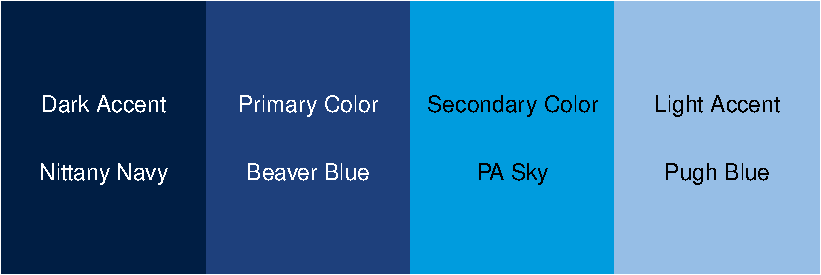
\includegraphics{BOAST_style_guide_files/figure-latex/bluePalette-1} 

}

\caption{The Blue Palette}\label{fig:bluePalette}
\end{figure}

\hypertarget{green}{%
\paragraph{Green}\label{green}}

The Green Palette looks like the following:

\begin{figure}

{\centering 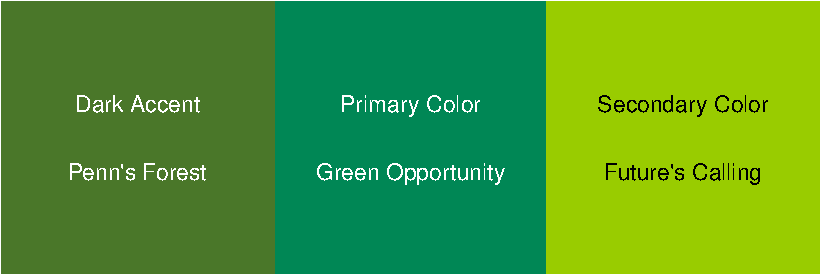
\includegraphics{BOAST_style_guide_files/figure-latex/greenPalette-1} 

}

\caption{The Green Palette}\label{fig:greenPalette}
\end{figure}

\hypertarget{purple}{%
\paragraph{Purple}\label{purple}}

The Purple Palette looks like the following:

\begin{figure}

{\centering 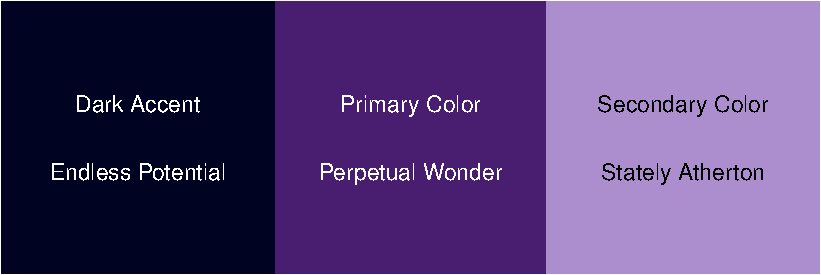
\includegraphics{BOAST_style_guide_files/figure-latex/purplePalette-1} 

}

\caption{The Purple Palette}\label{fig:purplePalette}
\end{figure}

\hypertarget{black}{%
\paragraph{Black}\label{black}}

The ``Black'' Palette is not pegged to the color black, but rather teal/aqua colors. However, to call the theme in the Shiny dashboard, the user must use the value \texttt{black} for the the \texttt{skin} argument. Here's what the ``Black'' Palette looks like:

\begin{figure}

{\centering 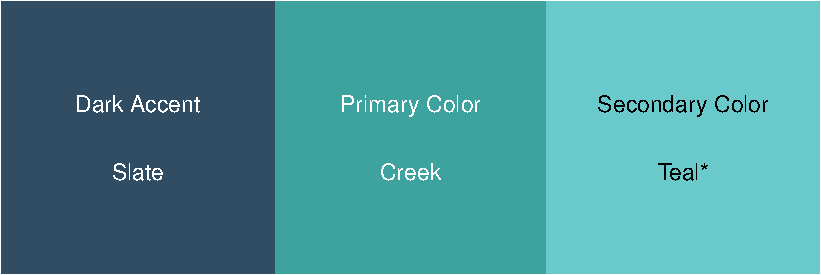
\includegraphics{BOAST_style_guide_files/figure-latex/blackPalette-1} 

}

\caption{The 'Black' Palette}\label{fig:blackPalette}
\end{figure}

\hypertarget{yellow}{%
\paragraph{Yellow}\label{yellow}}

The Yellow Palette is still under consideration. The current set looks like the following:

\begin{figure}

{\centering 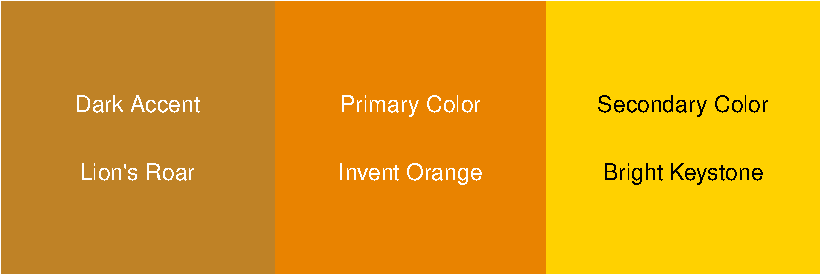
\includegraphics{BOAST_style_guide_files/figure-latex/yellowPalette-1} 

}

\caption{The Yellow Palette}\label{fig:yellowPalette}
\end{figure}

\hypertarget{red}{%
\paragraph{Red}\label{red}}

The Red Palette is still under construction. Here's the current set:

\begin{figure}

{\centering 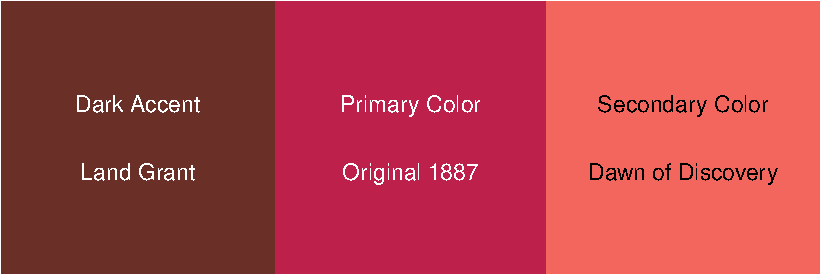
\includegraphics{BOAST_style_guide_files/figure-latex/redPalette-1} 

}

\caption{The Red Palette}\label{fig:redPalette}
\end{figure}

\hypertarget{color-and-plots-in-r}{%
\subsection{\texorpdfstring{Color and Plots in \texttt{R}}{Color and Plots in R}}\label{color-and-plots-in-r}}

In \texttt{R} you can set color theme which you use in \texttt{ggplot2}. Here are two custom color palettes that you can use in your App. Additionally, the package \texttt{viridis} provides several additional color palettes which are improvements upon the default color scheme.

\begin{Shaded}
\begin{Highlighting}[]
\CommentTok{# boastPalette is based on the Wong color blind set found at the above website.}
\NormalTok{boastPalette <-}\StringTok{ }\KeywordTok{c}\NormalTok{(}\StringTok{"#0072B2"}\NormalTok{,}\StringTok{"#D55E00"}\NormalTok{,}\StringTok{"#009E73"}\NormalTok{,}\StringTok{"#CE77A8"}\NormalTok{,}
    \StringTok{"#000000"}\NormalTok{,}\StringTok{"#E69F00"}\NormalTok{,}\StringTok{"#999999"}\NormalTok{,}\StringTok{"#56B4E9"}\NormalTok{,}\StringTok{"#CC79A7"}\NormalTok{)}

\CommentTok{# psuPalette is based on Penn State's three official color palettes}
\CommentTok{# and checked at the above webite.}
\NormalTok{psuPalette <-}\StringTok{ }\KeywordTok{c}\NormalTok{(}\StringTok{"#1E407C"}\NormalTok{,}\StringTok{"#BC204B"}\NormalTok{,}\StringTok{"#3EA39E"}\NormalTok{,}\StringTok{"#E98300"}\NormalTok{,}
    \StringTok{"#999999"}\NormalTok{,}\StringTok{"#AC8DCE"}\NormalTok{,}\StringTok{"#F2665E"}\NormalTok{,}\StringTok{"#99CC00"}\NormalTok{)}

\CommentTok{# Both palettes get used in the order of what is listed.}
\end{Highlighting}
\end{Shaded}

To use these palettes (or ones from \texttt{viridis}) with a \texttt{ggplot2} object, you'll need to doe the following

\begin{Shaded}
\begin{Highlighting}[]
\CommentTok{# You will need to first add whichever palette line from above to your code}
\NormalTok{boastPalette <-}\StringTok{ }\KeywordTok{c}\NormalTok{(}\StringTok{"#0072B2"}\NormalTok{,}\StringTok{"#D55E00"}\NormalTok{,}\StringTok{"#009E73"}\NormalTok{,}\StringTok{"#CE77A8"}\NormalTok{,}
    \StringTok{"#000000"}\NormalTok{,}\StringTok{"#E69F00"}\NormalTok{,}\StringTok{"#999999"}\NormalTok{,}\StringTok{"#56B4E9"}\NormalTok{,}\StringTok{"#CC79A7"}\NormalTok{)}

\CommentTok{# Create ggplot2 object}
\NormalTok{g1 <-}\StringTok{ }\NormalTok{ggplot2}\OperatorTok{::}\KeywordTok{ggplot}\NormalTok{(}\DataTypeTok{data =}\NormalTok{ df, }
                \KeywordTok{aes}\NormalTok{(}\DataTypeTok{x =}\NormalTok{ x, }\DataTypeTok{y =}\NormalTok{ y, }\DataTypeTok{color =}\NormalTok{ grp, }\DataTypeTok{fill =}\NormalTok{ grp))}
\CommentTok{# Add your layers}
\NormalTok{g1 }\OperatorTok{+}\StringTok{ }\NormalTok{ggplot2}\OperatorTok{::}\KeywordTok{geom_points}\NormalTok{()}
\CommentTok{# Tell R to use your chosen palette}
\NormalTok{g1 }\OperatorTok{+}\StringTok{ }\NormalTok{ggplot2}\OperatorTok{::}\KeywordTok{scale_color_manual}\NormalTok{(}\DataTypeTok{values=}\NormalTok{boastPalette)  }\CommentTok{# If you use "color" in aes}
\NormalTok{g1 }\OperatorTok{+}\StringTok{ }\NormalTok{ggplot2}\OperatorTok{::}\KeywordTok{scale_fill_manual}\NormalTok{(}\DataTypeTok{values=}\NormalTok{boastPalette)  }\CommentTok{# If you use "fill" in aes}
\end{Highlighting}
\end{Shaded}

If you have more groups than eight/nine colors listed in two palettes, consider reworking your examples as you could overwhelm the user with too many colors. (This also applies to using different shapes to plot points.)

\hypertarget{styleText}{%
\section{Text Styling}\label{styleText}}

Text styling refers the non-content aspects of the text on the page. This means things such as the use of italics, boldface, alignment, as well as font size and color.

You should let the centralized CSS file do the heavy lifting for text styling. (Again, using \texttt{boastApp} will help you.) However, for this to work properly, you will need to tag content appropriately. (See the HTML section: \ref{html})

If you run into a situation where some element needs additionl styling, \textbf{talk to Neil or Bob for help}. You might have come across an element that needs to get added the central CSS file or a bug.

\hypertarget{headings}{%
\subsection{Headings}\label{headings}}

Use the Heading Tags for the short fragments that define the structure of your App. If you find yourself enclosing a complete sentence in Heading tag, you ARE NOT using headings correctly. Notice how the headings in this Style Guide aren't complete sentences; your App should mimic this. Full sentences appear as regular paragraph text (i.e., enclosed in \texttt{p()}) and not be a Heading.

\hypertarget{paragraph-text}{%
\subsection{Paragraph Text}\label{paragraph-text}}

If you enclose text that gives instructions or other information to your App's users in \texttt{p()} or \texttt{li()} (the later should be wrapped in either \texttt{tags\$ol()} or \texttt{tags\$ul()}), your App will understand how to style that text correctly. The central CSS file contains controls that set the base font size much larger than Shiny does natively as well as making text sizing dynamic. (This is important for making our apps mobile device friendly.) Again, using \texttt{boastApp} makes this process easier.

If you want to make a certain word or phrase italic, you will need to wrap that text in \texttt{tags\$em()}. Similarly, if you want do the same with boldface, you'll use \texttt{tags\$strong()}.

For example, this code:

\begin{Shaded}
\begin{Highlighting}[]
\KeywordTok{p}\NormalTok{(}
  \StringTok{"When dealing with the "}\NormalTok{,}
\NormalTok{  tags}\OperatorTok{$}\KeywordTok{em}\NormalTok{(}\StringTok{"t"}\NormalTok{),}
  \StringTok{"-distribution, we only have one parameter, the "}\NormalTok{,}
\NormalTok{  tags}\OperatorTok{$}\KeywordTok{strong}\NormalTok{(}\StringTok{"degrees of freedom"}\NormalTok{),}
  \StringTok{"that we need to input."}
\NormalTok{)}
\end{Highlighting}
\end{Shaded}

Becomes:

\begin{quote}
When dealing with the \emph{t}-distribution, we only have one parameter, the \textbf{degrees of freedom} that we need to input.
\end{quote}

Use italics (emphasis), and boldface (strong) sparingly.

\hypertarget{mathematics}{%
\subsection{Mathematics}\label{mathematics}}

For the most part, any mathematics you need displayed should be done using \href{https://www.mathjax.org/}{MathJax}. Default to using inline typesetting with the \texttt{\textbackslash{}\textbackslash{}(} and \texttt{\textbackslash{}\textbackslash{})} delimiters. If you need to use display style, you can use \texttt{\textbackslash{}\textbackslash{}{[}} and \texttt{\textbackslash{}\textbackslash{}{]}}. For the vast majority of mathematics, you'll wrap both inline and display style mathematics inside of a paragraph environment (\texttt{p()}).

If you're writing mathematics directly in your app, remember you'll need to escape the LaTeX commands by putting an extra backslash (\textbackslash{}) in front; e.g., \texttt{\textbackslash{}frac\{3\}\{4\}} would need to be \texttt{\textbackslash{}\textbackslash{}frac\{3\}\{4\}}.

If you're reading in mathematical text from an external CSV file, you do not need the extra backslash in the CSV file.

\textbf{Note:} Double dollar sign delimiters are generally not recommended for displaying math as they can lead to unintended results. See: \href{https://docs.mathjax.org/en/latest/basic/mathematics.html}{Writing Mathematics for MathJax}.

\hypertarget{game-question-text}{%
\subsection{{[}Game{]} Question Text}\label{game-question-text}}

The text used as a question in a game should NOT be wrapped in a Heading tag; wrap the text in a paragraph tag.

\hypertarget{label-text-buttons-sliders-other-inputs-and-alerts}{%
\subsection{Label Text (Buttons, Sliders, Other Inputs and Alerts)}\label{label-text-buttons-sliders-other-inputs-and-alerts}}

By using the central CSS file, any text you included in/on buttons, dropdown menus, sliders, radio buttons, choices, and other inputs as well as alert messages and popups/rollovers, will automatically be styled correctly.

Do not use heading tags, the paragraph tag, italics/emphasis, or boldface/strong with input labels.

You may use these tags with popups/rollovers.

\hypertarget{feedback-and-hint-text}{%
\subsection{Feedback and Hint Text}\label{feedback-and-hint-text}}

Again, let the central CSS file handle the styling of this type of text.

\hypertarget{text-in-r-plots}{%
\subsection{\texorpdfstring{Text in \texttt{R} Plots}{Text in R Plots}}\label{text-in-r-plots}}

Unfortunately, any text in \texttt{R} plots does not get controlled by CSS. This means that you'll have to play around with the settings. Using the \texttt{ggplot2} package to make your plots (or other packages based upon the ggplot framework) will allow you to use the \texttt{theme} aspect to control text in your App.

Here is an example for how to do this:

\begin{Shaded}
\begin{Highlighting}[]
\CommentTok{# Create a ggplot2 object}
\NormalTok{g1 <-}\StringTok{ }\NormalTok{ggplot2}\OperatorTok{::}\KeywordTok{ggplot}\NormalTok{(}\DataTypeTok{data=}\NormalTok{df, }\KeywordTok{aes}\NormalTok{(}\DataTypeTok{x=}\NormalTok{x, }\DataTypeTok{y=}\NormalTok{y, }\DataTypeTok{color=}\NormalTok{grp)) }
\CommentTok{# Add your layers, for example}
\NormalTok{g1 }\OperatorTok{+}\StringTok{ }\NormalTok{ggplot2}\OperatorTok{::}\KeywordTok{geom_point}\NormalTok{()}
\CommentTok{# Use theme to control text size}
\NormalTok{g1 }\OperatorTok{+}\StringTok{ }\NormalTok{ggplot2}\OperatorTok{::}\KeywordTok{theme}\NormalTok{(}
  \DataTypeTok{plot.caption =} \KeywordTok{element_text}\NormalTok{(}\DataTypeTok{size =} \DecValTok{18}\NormalTok{),}
  \DataTypeTok{text =} \KeywordTok{element_text}\NormalTok{(}\DataTypeTok{size =} \DecValTok{18}\NormalTok{)}
\NormalTok{  )}
\end{Highlighting}
\end{Shaded}

You will need to play around with the settings to find the appropriate value; text size 18 appears to work out well in many cases.

\textbf{Note:} The text in your plot might not behave well for dynamic resizing on different mobile devices.

\hypertarget{graphics}{%
\section{Graphics}\label{graphics}}

One of the most powerful tools we have in Statistics and Data Science is graphics. This includes images/pictures, graphs/plots, and tables. You will want to make sure that all graphical elements are appropriately sized in the Body. If there is text in a static image/picture, you'll need to make sure that the text is legible on a variety of screen sizes.

We've already discussed both issues of color and text size in plots. For additional considerations, please refer to the following readings (ordered from most important to least):

\begin{itemize}
\tightlist
\item
  \href{https://www.dropbox.com/s/hb52991v09p8q91/Tufte\%20-\%202006\%20-\%20The\%20Fundamental\%20principles\%20of\%20analytical\%20design.pdf?dl=0}{Tufte-Fundamental Principles of Analytical Design}
\item
  \href{https://www.dropbox.com/s/z8yrf4eqph6c2h4/Tufte\%20-\%202001\%20-\%20Chartjunk\%20Vibrations\%2C\%20grids\%2C\%20and\%20ducks.pdf?dl=0}{Tufte-Chartjunk}\\
\item
  \href{https://www.dropbox.com/s/62uegsribwdjtze/Kosslyn\%20-\%202006\%20-\%20Looking\%20with\%20the\%20eye\%20and\%20mind.pdf?dl=0}{Kosslyn-Looking with the Eye and Mind}
\end{itemize}

Remember, we always want to be modeling excellent graphing behaviors.

\begin{quote}
All photographs can be fortified with words. --Dorothea Lange
\end{quote}

\begin{quote}
A picture is worth a thousand words\ldots{}but which ones. --Unknown
\end{quote}

Both of these quotations highlight that you need to include some text with your plots to help the user construct their understanding of what you're trying to show them.

\hypertarget{axes-and-scales}{%
\subsection{Axes and Scales}\label{axes-and-scales}}

\texttt{R}'s default axes are terrible. They often do not fully cover the data and the have gaps between the axes. All this impedes the user's construction of meaning. Thus, you'll want to take control and stipulate the axes and scales to optimize what users get out of the plot. If you are providing multiple plots that the user is supposed to compare, make sure that they all use the same scaling and axes.

To force \texttt{ggplot2} to place (0, 0) in the lower-left corner and to control the scales, you will need to include the following:

\begin{Shaded}
\begin{Highlighting}[]
\CommentTok{# Create the ggplot2 object}
\NormalTok{g1 <-}\StringTok{ }\NormalTok{ggplot2}\OperatorTok{::}\KeywordTok{ggplot}\NormalTok{(...)}
\CommentTok{# Add your layer}
\NormalTok{g1 }\OperatorTok{+}\StringTok{ }\NormalTok{ggplot2}\OperatorTok{::}\KeywordTok{geom_point}\NormalTok{()}
\CommentTok{# Control axes and scale}
\CommentTok{## Multplicative Scaling of the Horizontal (x) Axis}
\CommentTok{## Additive Scaling of the Vertical (y) Axis}
\NormalTok{g1 }\OperatorTok{+}\StringTok{ }\NormalTok{ggplot2}\OperatorTok{::}\KeywordTok{scale_x_continuous}\NormalTok{(}\DataTypeTok{expand =} \KeywordTok{expansion}\NormalTok{(}\DataTypeTok{mult =} \KeywordTok{c}\NormalTok{(}\DecValTok{1}\NormalTok{,}\DecValTok{2}\NormalTok{), }\DataTypeTok{add =} \DecValTok{0}\NormalTok{)) }\OperatorTok{+}\StringTok{ }
\StringTok{  }\KeywordTok{scale_y_continuous}\NormalTok{(}\DataTypeTok{expand =} \KeywordTok{expansion}\NormalTok{(}\DataTypeTok{mult =} \DecValTok{0}\NormalTok{, }\DataTypeTok{add =} \KeywordTok{c}\NormalTok{(}\DecValTok{0}\NormalTok{,}\FloatTok{0.05}\NormalTok{))) }
\end{Highlighting}
\end{Shaded}

\hypertarget{tables}{%
\subsection{Tables}\label{tables}}

Use tables as infrequently as possible. If you absolutely must include a table, you will need to decide what the role of your table is. This is an Accessibility issue that you \textbf{MUST} pre-plan for. Screen readers will poorly communicate tables if you fail to set the role appropriately. \textbf{Talk to Neil and Bob} before using a table.

\hypertarget{alt-text}{%
\subsection{Alt Text}\label{alt-text}}

Any graphical element you include in your App \textbf{MUST} have an alternative (assistive) text description (``alt text''). This provides a short description of what is in the image or plot for users who are visual impaired. (Tables, when properly formated will handle this automatically.)

\hypertarget{miscellaneous}{%
\section{Miscellaneous}\label{miscellaneous}}

Consider adding a loading bar to show the process for intense computations; this will help the user understand that your App is processing and not frozen/broken.

\hypertarget{wording}{%
\chapter{Wording}\label{wording}}

\hypertarget{general-guidelines}{%
\section{General Guidelines}\label{general-guidelines}}

When writing the content for your App, you will want to keep in mind that these app have the primary audience of students. Thus, we need to make sure that we use language that is appropriate. Seek to use complete sentences that convey what you intend. Have someone else take a look at your content and then tell you what they believe the text to be saying. If what they say is consistent with what you intended, great. If not, then you need to revise your text.

\textbf{DO NOT sacrifice clarity and precision/accuracy for
conciseness/brevity.}

Since these apps are for \emph{teaching}, we need to use language that is accurate and supports students in constructing productive meanings. This means that we need to avoid sloppy language, re-enforcing problematic conceptions, and supporting fallacies. For example,

\begin{itemize}
\tightlist
\item
  Discussing values of statistics

  \begin{itemize}
  \tightlist
  \item
    BAD: ``The mean is 6.''
  \item
    GOOD: ``The value of the \emph{sample arithematic mean} for this data is 6 units/object.''
  \end{itemize}
\item
  Problematic conceptions

  \begin{itemize}
  \tightlist
  \item
    BAD: ``Probability is the likelihood of an event in relation to all possible events.''
  \item
    GOOD: ``Probability is the long-run relative frequency for us seeing a particular data event given our assumptions. Likelihood is the long-run relative frequency of a set of assumptions being true given our collected data.''
  \end{itemize}
\item
  Fallacies

  \begin{itemize}
  \tightlist
  \item
    BAD: ``We're 95\% confident that the true population proportion is between 0.35 and 0.45.''
  \item
    GOOD: ``If we were to repeat the entire study infinitely many times, then 95\% of the time we will make an interval that captures the true population proportion.''
  \end{itemize}
\end{itemize}

\hypertarget{popovers}{%
\section{Popovers}\label{popovers}}

Popovers refers to any number of different tools on websites that go by other names such as tooltips, rollovers, and hover text. In essence, this tool appears when the user places their cursor over (i.e., hover) or shifts the focus to a trigger object. The text then pops up on the screen for the user to view. The function to create one of these in a Shiny app is \texttt{shinyBS::bsPopover}. While these can be powerful, they are often misused which leads to problems. For example, they can prevent the user from actually interacting with portions of your app when they appear.

Popovers are meant to provide short, simple clarifications; quick annotations which enrich the content that is already present. This type of text is meant to be temporary, only appearing for as long as the user is hovering/focusing on the trigger object. Thus, if you are putting information that is critical to your user successfully using your App in a popover, you are using popovers \textbf{INCORRECTLY}.

Here are few additional sources for reading about Popovers/Tooltips:

\begin{itemize}
\tightlist
\item
  \href{https://uxplanet.org/tooltips-in-ui-design-f63e117aa3d1}{Tooltips in UI Design}
\item
  \href{https://www.appcues.com/blog/tooltips}{Tooltips: How to use this small but mighty UI pattern correctly}
\end{itemize}

Restrict any usage of a popover to something short and non-vital for your App's user. If you do choose to use a popover, you will need to format the popover correctly. Be sure that your function call includes values for the following arguments:

\begin{itemize}
\tightlist
\item
  \texttt{id}: this needs to be the name of the object which will act as the trigger
\item
  \texttt{title}: this will be a string that appears across the top of your popover; use verbs with an understood ``you'' (e.g., ``Investigate!'', ``Remember'', etc.)
\item
  \texttt{content}: this will be the string that you want displayed; shorter is better.
\item
  \texttt{placement}: this will control where the popover appears. Choose the option (top, bottom, left, right) that works best for your space. Ensure that the placement does not cover any controls or other vital information.
\end{itemize}

\hypertarget{documentation}{%
\chapter{Documentation}\label{documentation}}

These apps are the product of your hardwork and are part of your academic record. Thus, you need to adhere to \href{https://undergrad.psu.edu/aappm/G-9-academic-integrity.html}{Penn State's Academic Integrity Policy}. This is especially important as we are making the apps available through a Creative Commons Attribution-ShareAlike 4.0 International license (\href{https://creativecommons.org/licenses/by-sa/4.0/}{CC BY-SA 4.0}). If you have used code, pictures, data, or other materials from outside of the BOAST team, you \textbf{MUST} give proper credit. These references will then be included on the App's References Tab.

\hypertarget{references-1}{%
\section{References}\label{references-1}}

All apps will need a References Tab. This is where you'll place all references for your App, including R packages, borrowed code, data sources, images, etc. This in addition to the Acknowledgements. (NOTE: listing something in the Acknowledgements DOES NOT waive this requirement.)

You may use any citation style you wish, but be consistent. Recommended citation styles include APA and AmStat. Here is a starting code block for you to use:

\begin{Shaded}
\begin{Highlighting}[]
\CommentTok{#[omitted code]}
\KeywordTok{tabItem}\NormalTok{(}
  \DataTypeTok{tabName =} \StringTok{"refs"}\NormalTok{,}
  \KeywordTok{withMathJax}\NormalTok{(),}
  \KeywordTok{h2}\NormalTok{(}\StringTok{"References"}\NormalTok{),}
  \KeywordTok{p}\NormalTok{(}\DataTypeTok{class =} \StringTok{"hangingindent"}\NormalTok{,}
    \StringTok{"reference 1-alphabetically"}\NormalTok{),}
  \KeywordTok{p}\NormalTok{(}\DataTypeTok{class =} \StringTok{"hangingindent"}\NormalTok{,}
    \StringTok{"reference 2-alphabetically"}\NormalTok{),}
  \CommentTok{# Repeat as needed}
\NormalTok{)}
\end{Highlighting}
\end{Shaded}

If you need assistance with this section, please talk to Neil.

\hypertarget{plagiarism}{%
\section{Plagiarism}\label{plagiarism}}

\textbf{You MAY NOT use blocks of code you've found online without giving proper attribution.}

There is a difference between looking at example code online to see how to do something and copying that code directly. The former is permissible, the later is plagiarism.

\begin{itemize}
\tightlist
\item
  If you want to use someone else's code ``as is'' (without any changes), you should reach out to the author for permission first.
\item
  If you use someone else's code and make modifications, you need to give credit to where you got the code, and potentially ask for permission.
\end{itemize}

You will need to place citations in \emph{\textbf{two}} places: in the References Tab and in your code.

\hypertarget{reference-tab}{%
\subsection{Reference Tab}\label{reference-tab}}

Use the following format:

\begin{quote}
Author. (Date). Title of program/source code (Version number, if applicable). {[}type of code{]}. Retrieved from \textless{} URL \textgreater{}.
\end{quote}

For example,

\begin{quote}
Hatfield, N. J. (2017). First day activity (v1). {[}Netlogo{]}. Retrieved from \url{https://neilhatfield.github.io/statApps/Day1Activity.html}.
\end{quote}

\hypertarget{in-code}{%
\subsection{In Code}\label{in-code}}

Use the following format in your code to cite where you got the code from.

\begin{Shaded}
\begin{Highlighting}[]
\CommentTok{#-------------------------------------------------------------------------------}
\CommentTok{#  Title: <title of program/source code>}
\CommentTok{#  Author: <author(s) names>}
\CommentTok{#  Date: <date>}
\CommentTok{#  Code version: <code version>}
\CommentTok{#  Availability: <where it's located>}
\CommentTok{#-------------------------------------------------------------------------------}
\CommentTok{# [borrowed code then follows]}
\CommentTok{# ...}
\CommentTok{# [last line of borrowed code]      }
\CommentTok{#End of <author>'s code-------------------------------------------------------------------}
\end{Highlighting}
\end{Shaded}

\hypertarget{r-packages}{%
\section{\texorpdfstring{\texttt{R} Packages}{R Packages}}\label{r-packages}}

If you made use of any packages in \texttt{R}, then you will need to add these to the Reference subsection. Fortunately, there is a built-in tool that will help you: the \texttt{citation} function. In R (RStudio) simply type \texttt{citation("packageName")} and you'll get the appropriate citation information for the package you used. For example, \texttt{citation("shinydashboard")} and \texttt{citation("plyr")} will give the information needed for the following citations:

\begin{quote}
Chang, W. and Borges Ribeio, B. (2018). shinydashboard: Create dashboards with `Shiny'. (v0.7.1) {[}R Package{]}. Available from \url{https://CRAN.R-project.org/package=shinydashboard}
\end{quote}

\begin{quote}
Wickham, H. (2011). The Split-apply-combine strategy for data analysis. Journal of Statistical Software, 40(1). pp.~1-29. Available at \url{http://www.jstatsoft.org/v40/i01/}.
\end{quote}

Notice, that the format of the R package will depend on whether there is an article published for the package. The \texttt{shinydashboard} package is not associated with an article while the \texttt{plyr} package is associated with Wickham's article.

\hypertarget{graphics-1}{%
\section{Graphics}\label{graphics-1}}

Pictures, drawings, photographs, images, etc. are typically copyrighted. When you're selecting images, make sure that the images are Open Source/Copyright Free/Royalty Free/Public Domain. Additionally, include a reference to where the pictures came from in the Overview Page. The basic format to use is:

\begin{quote}
LastName, First Initial. (Year). Title of artwork. {[}Format{]}. Retrieved from \textless{} URL \textgreater{}.
\end{quote}

\hypertarget{data}{%
\section{Data}\label{data}}

If you are using any data files, you need to attribute where those files are coming from in the References subsection of your Overview page. A suggested format to use is:

\begin{quote}
Author/Rightsholder. (Year). Title of data set (Version number) {[}Description of form{]}. Location: Name of producer.
\end{quote}

\begin{quote}
Author/Rightsholder. (Year). Title of data set (Version number) {[}Description of form{]}. Retrieved from \url{http://www.url.com}
\end{quote}

If you (or someone else) had to sign some type of agreement to access the data, we must examine the agreement before you make your App publicly accessible. Just because you got access to the data does not mean you have the right to share the data.

\hypertarget{accessibility}{%
\chapter{Accessibility}\label{accessibility}}

We need to make sure that our Apps are accessible. If you have been adhering to the style guide, your App should be in a decent position. When you're ready to test the accessibility of your App, you'll need to deploy the App to a sever and then use the \href{https://wave.webaim.org/}{WAVE Web Accessibility Evaluation Tool}. Enter the URL of your App in the noted box to run an evaluation. See what accessibility issues your App has and then address them.

\textbf{See also:}

\begin{itemize}
\tightlist
\item
  \href{https://accessibility.psu.edu/}{Accessibility and Usability at Penn
  State}
\item
  \href{https://www.psu.edu/accessibilitystatement}{Accessibility
  Statement}
\item
  \href{https://www.w3.org/WAI/WCAG21/quickref/}{How to Meet Web Content Accessibility
  Guidelines}
\item
  \href{https://medium.com/salesforce-ux/7-things-every-designer-needs-to-know-about-accessibility-64f105f0881b}{7 Things Every Designer Needs to Know about Accessibility}
\end{itemize}

\hypertarget{mobile}{%
\chapter{Mobile Friendliness}\label{mobile}}

We want our apps to work well with mobile devices. Thus, when you get to the point where the majority of bugs have been fixed, you need to check how mobile friendly your App is. If you have used \texttt{boastApp} and/or the \texttt{boast.CSS} file, along with the practices laid out earlier, then you should be well on your way to being mobile friendly.

You can check your App in two ways:

\begin{enumerate}
\def\labelenumi{\arabic{enumi}.}
\tightlist
\item
  Test your App out on a variety of mobile devices.
\item
  Make use of a browser's ability to mimic devices. To do this, launch your App in a browser, then enable one of the following:

  \begin{itemize}
  \tightlist
  \item
    \href{https://developers.google.com/web/tools/chrome-devtools/device-mode/\#viewport}{Chrome: Device Mode}
  \item
    \href{https://developer.mozilla.org/en-US/docs/Tools/Responsive_Design_Mode}{Firefox: Responsive Design Mode}
  \item
    \href{https://docs.microsoft.com/en-us/microsoft-edge/devtools-guide/emulation}{Microsoft Edge: Device Emulation}
  \item
    \href{https://support.apple.com/en-gb/guide/safari-developer/dev84bd42758/mac}{Safari: Responsive Design Mode}
  \end{itemize}
\end{enumerate}

Look for any issues that you might be able to address before you hand off your App for others to play around with. Assign a \textbf{Mobile Friendliness Rating} to your App on a scale from 1 to 5.

\begin{enumerate}
\def\labelenumi{\arabic{enumi}.}
\tightlist
\item
  Not functional
\item
  Functional -- Very awkward
\item
  Functional -- Okay if no big screen available (multiple issues)
\item
  Usable in a small class setting (single issue)
\item
  Readily usable
\end{enumerate}

\hypertarget{addTools}{%
\chapter{Additional Tools}\label{addTools}}

Here are a few additional tools that can help you with App development.

\begin{itemize}
\tightlist
\item
  \href{https://github.com/jimhester/lintr}{lintr} - Checks adherence to a
  given style, syntax errors, and possible semantic issues.
\item
  \href{https://www.tidyverse.org/articles/2017/12/styler-1.0.0/}{styler} -
  Format R code according to a style guide.
\item
  \href{https://github.com/MichaelChirico/funchir}{funchir} - stale package
  check
\end{itemize}

\bibliography{book.bib,packages.bib}

\end{document}
